\chapter{Modelado y construcción del PCB.}
% ----------------------

\label{C:EModelado y construcción del PCB.}

\section{Software y herramientas de diseño empleadas.}

A partir de los circuitos desarrollados en los capítulos anteriores, se procedió a diseñar una placa de circuito impreso (PCB) personalizada. Esta placa está diseñada para integrar todos los componentes necesarios y crear un prototipo funcional que permita realizar ensayos sobre materiales en una superficie comprimida. La modelación y diseño del PCB se llevó a cabo utilizando el software KiCad, reconocido por su amplia gama de herramientas de personalización de componentes. Este software permite a los diseñadores lograr un alto nivel de precisión y calidad en sus diseños, adecuándose a las habilidades específicas de cada usuario.\cite{kicad} \par 
El proceso de diseño del (PCB) incluyó la disposición estratégica de los componentes para optimizar el rendimiento del circuito, así como la consideración de factores como la disipación de calor, la integridad de la señal y la minimización de interferencias electromagnéticas. Además, se realizaron varias iteraciones del diseño para asegurar que el PCB final cumpliera con todos los requisitos técnicos y de funcionamiento necesarios para los ensayos planificados. \par 
El uso de KiCad facilitó la creación de un diseño detallado y eficiente, permitiendo visualizar en todo momento el aspecto final del PCB y realizar ajustes necesarios antes de proceder a su fabricación.\par
A su vez para realizar los ensayos del código del microcontrolador, se empleó el software de simulación de circuitos electrónicos \textit{Proteus 8 Professional}. Este programa ofrece un conjunto de herramientas avanzadas que facilitan la evaluación del comportamiento de los componentes integrados en el control digital, permitiendo compararlos con modelos teóricos de manera eficiente. Además, \textit{Proteus 8 Professional} permite la carga directa de archivos de código en microcontroladores ficticios, lo que posibilita la simulación completa del sistema y el análisis de su desempeño en condiciones virtuales antes de su implementación física.


\section{Ensayos y simulación de periféricos}
Una de las características más destacadas de \entreComillas{Proteus 8 Professional}, y la razón principal por la que se prefiere frente a otras alternativas, es su comunidad activa. Esta comunidad ha desarrollado librerías extensivas de componentes, incluidos microcontroladores Arduino. Estas librerías no solo incluyen las huellas (footprints) de los componentes, sino que también permiten programarlos de manera similar a como se haría con los dispositivos reales. Esta funcionalidad es particularmente valiosa, ya que permite al diseñador observar una simulación precisa de la interacción entre todos los elementos, sirviendo como base para la implementación con componentes físicos en etapas posteriores del desarrollo.\par

En la Figura \ref{F:esquematico_proteus} se presenta resumidamente la etapa de control de periféricos del proyecto, indicando la interconexión de los distintos módulos al microcontrolador.\par
\begin{figure}[H]
    \centering
    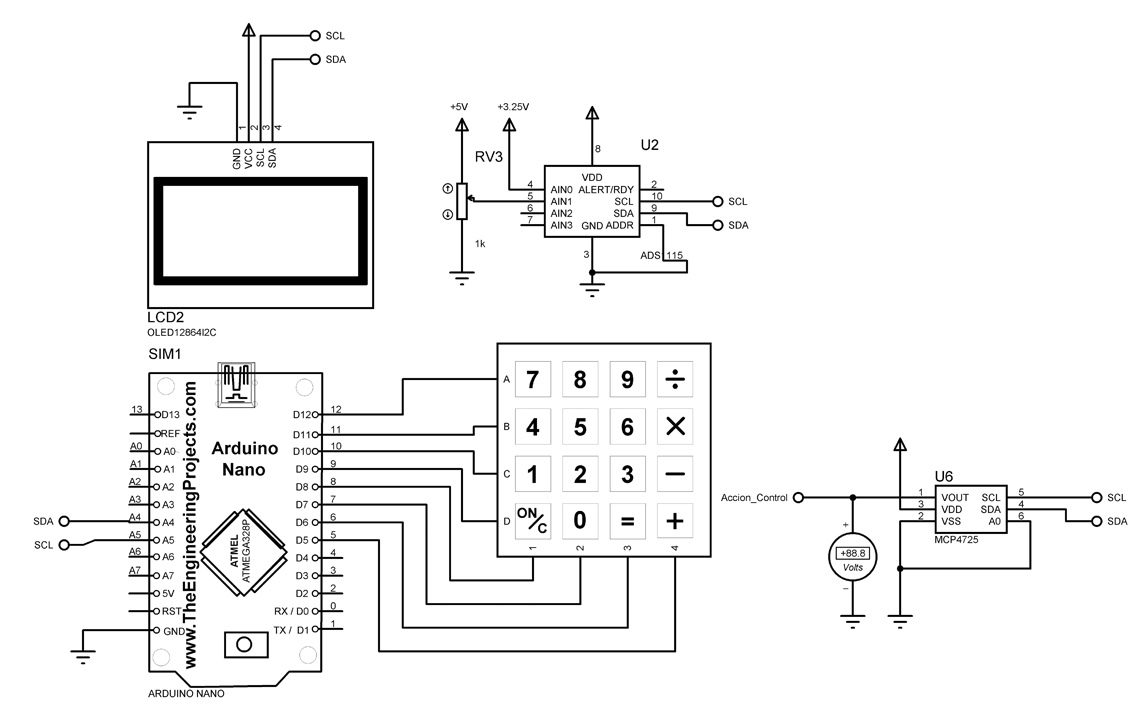
\includegraphics[width=\textwidth]{./imagenes/proteus_esquema2.jpg}
    \caption{Esquemático de conexión de los componentes digitales para un primer ensayo.}
    \label{F:esquematico_proteus}
\end{figure}

\subsection{Resultados experimentales de periféricos}
Basado en el desarrollo descrito en la sección anterior, se obtuvo un modelo funcional de circuito y código que cumplía con los objetivos propuestos del sistema de control. Esto culminó en el ensayo físico de los componentes utilizando una base \textit{protoboard}, donde se comprobó que todos los elementos funcionaron, siguiendo el esquema provisto en la Figura \ref{F:ensayo_digital}. Así, se concluyó exitosamente el ensayo de esta sección, validando el diseño y su implementación práctica.\par
\begin{foto}[H]
    \centering
    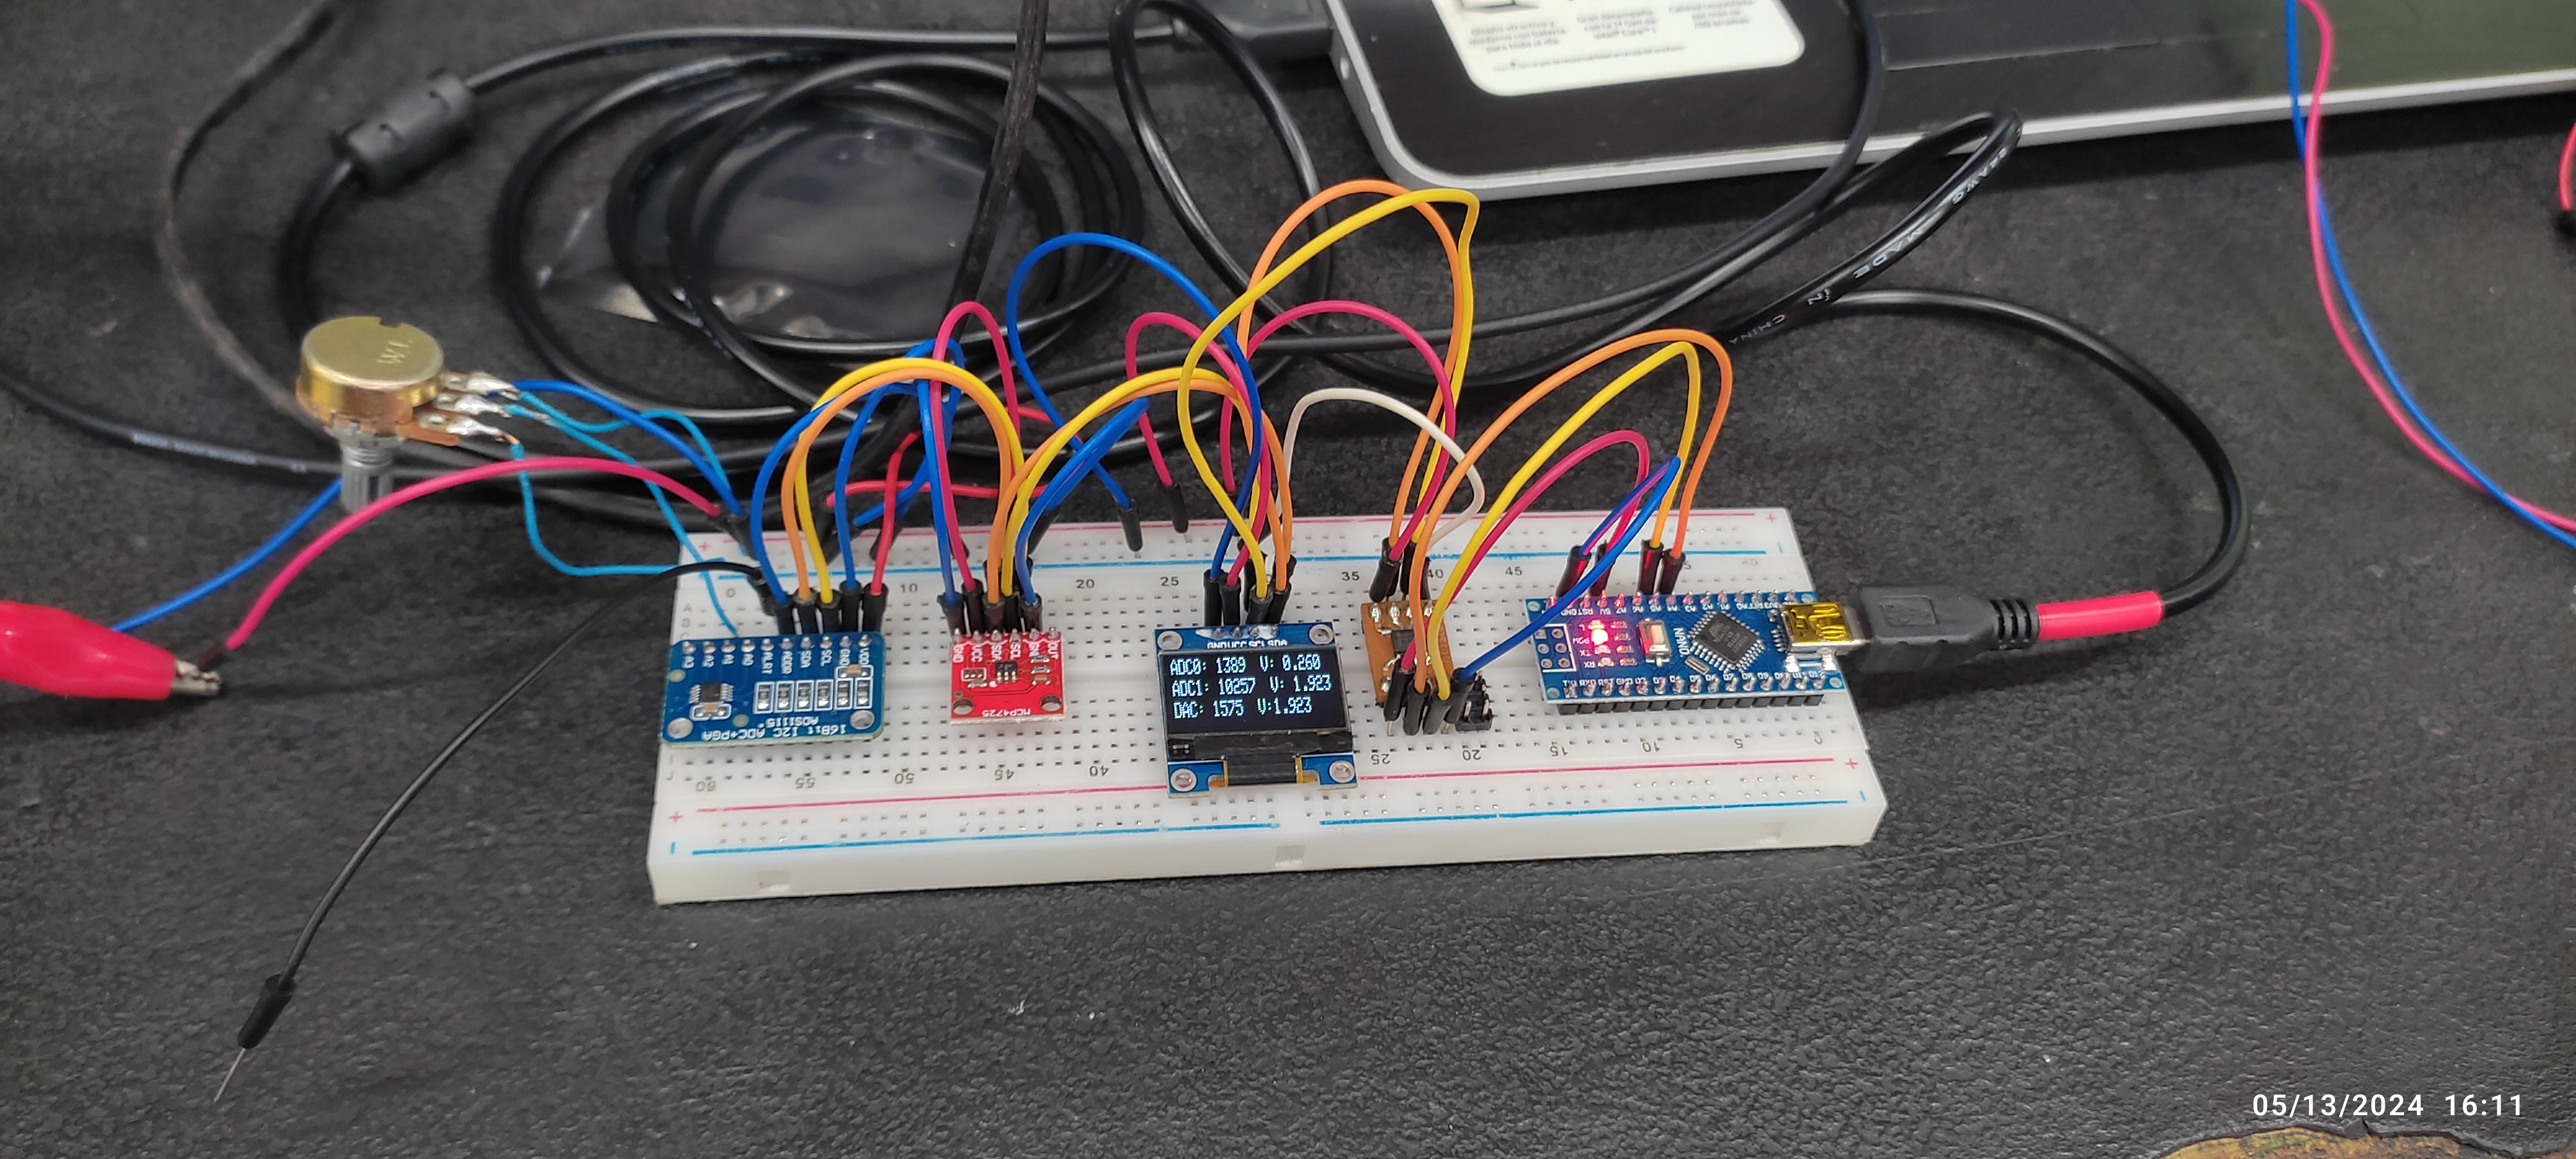
\includegraphics[scale=0.08]{./imagenes/ensayo_digital.jpg}
    \caption{Ensayo en \textit{protoboard} de los componentes correspondientes a la etapa digital.}
    \label{F:ensayo_digital}
\end{foto}

\section{Construcción del primer prototipo.}
La fase de construcción se inició con el desmontaje de la placa analógica de la fuente utilizada en un proyecto anterior que se puede apreciar en la fotografía \ref{F:placa_original}, la cual se caracterizaba por sus atributos de control predominantemente analógicos. Este proceso permitió la recuperación de una variedad de materiales que, en su mayoría, se emplearían en el desarrollo del nuevo prototipo de fuente digital. Entre los componentes rescatados se encuentran resistencias, capacitores, disipadores de calor, borneras, entre otros. La reutilización de estos elementos fue posible gracias a la topología de la nueva fuente digital, que permitía su integración sin comprometer el diseño ni la funcionalidad del prototipo.  \par 
El proceso de desmontaje y reutilización de componentes se llevó a cabo meticulosamente, asegurando que cada pieza recuperada estuviera en condiciones óptimas para su reincorporación como se observa en la fotografía \ref{F:desmontaje_de_la_placa}. Este esfuerzo contribuyó a la eficiencia del proyecto y a la racionalización de recursos, destacando la importancia de la sostenibilidad y la economía circular en el ámbito del diseño y construcción de dispositivos electrónicos.\par
\begin{foto}[H]
    \centering
    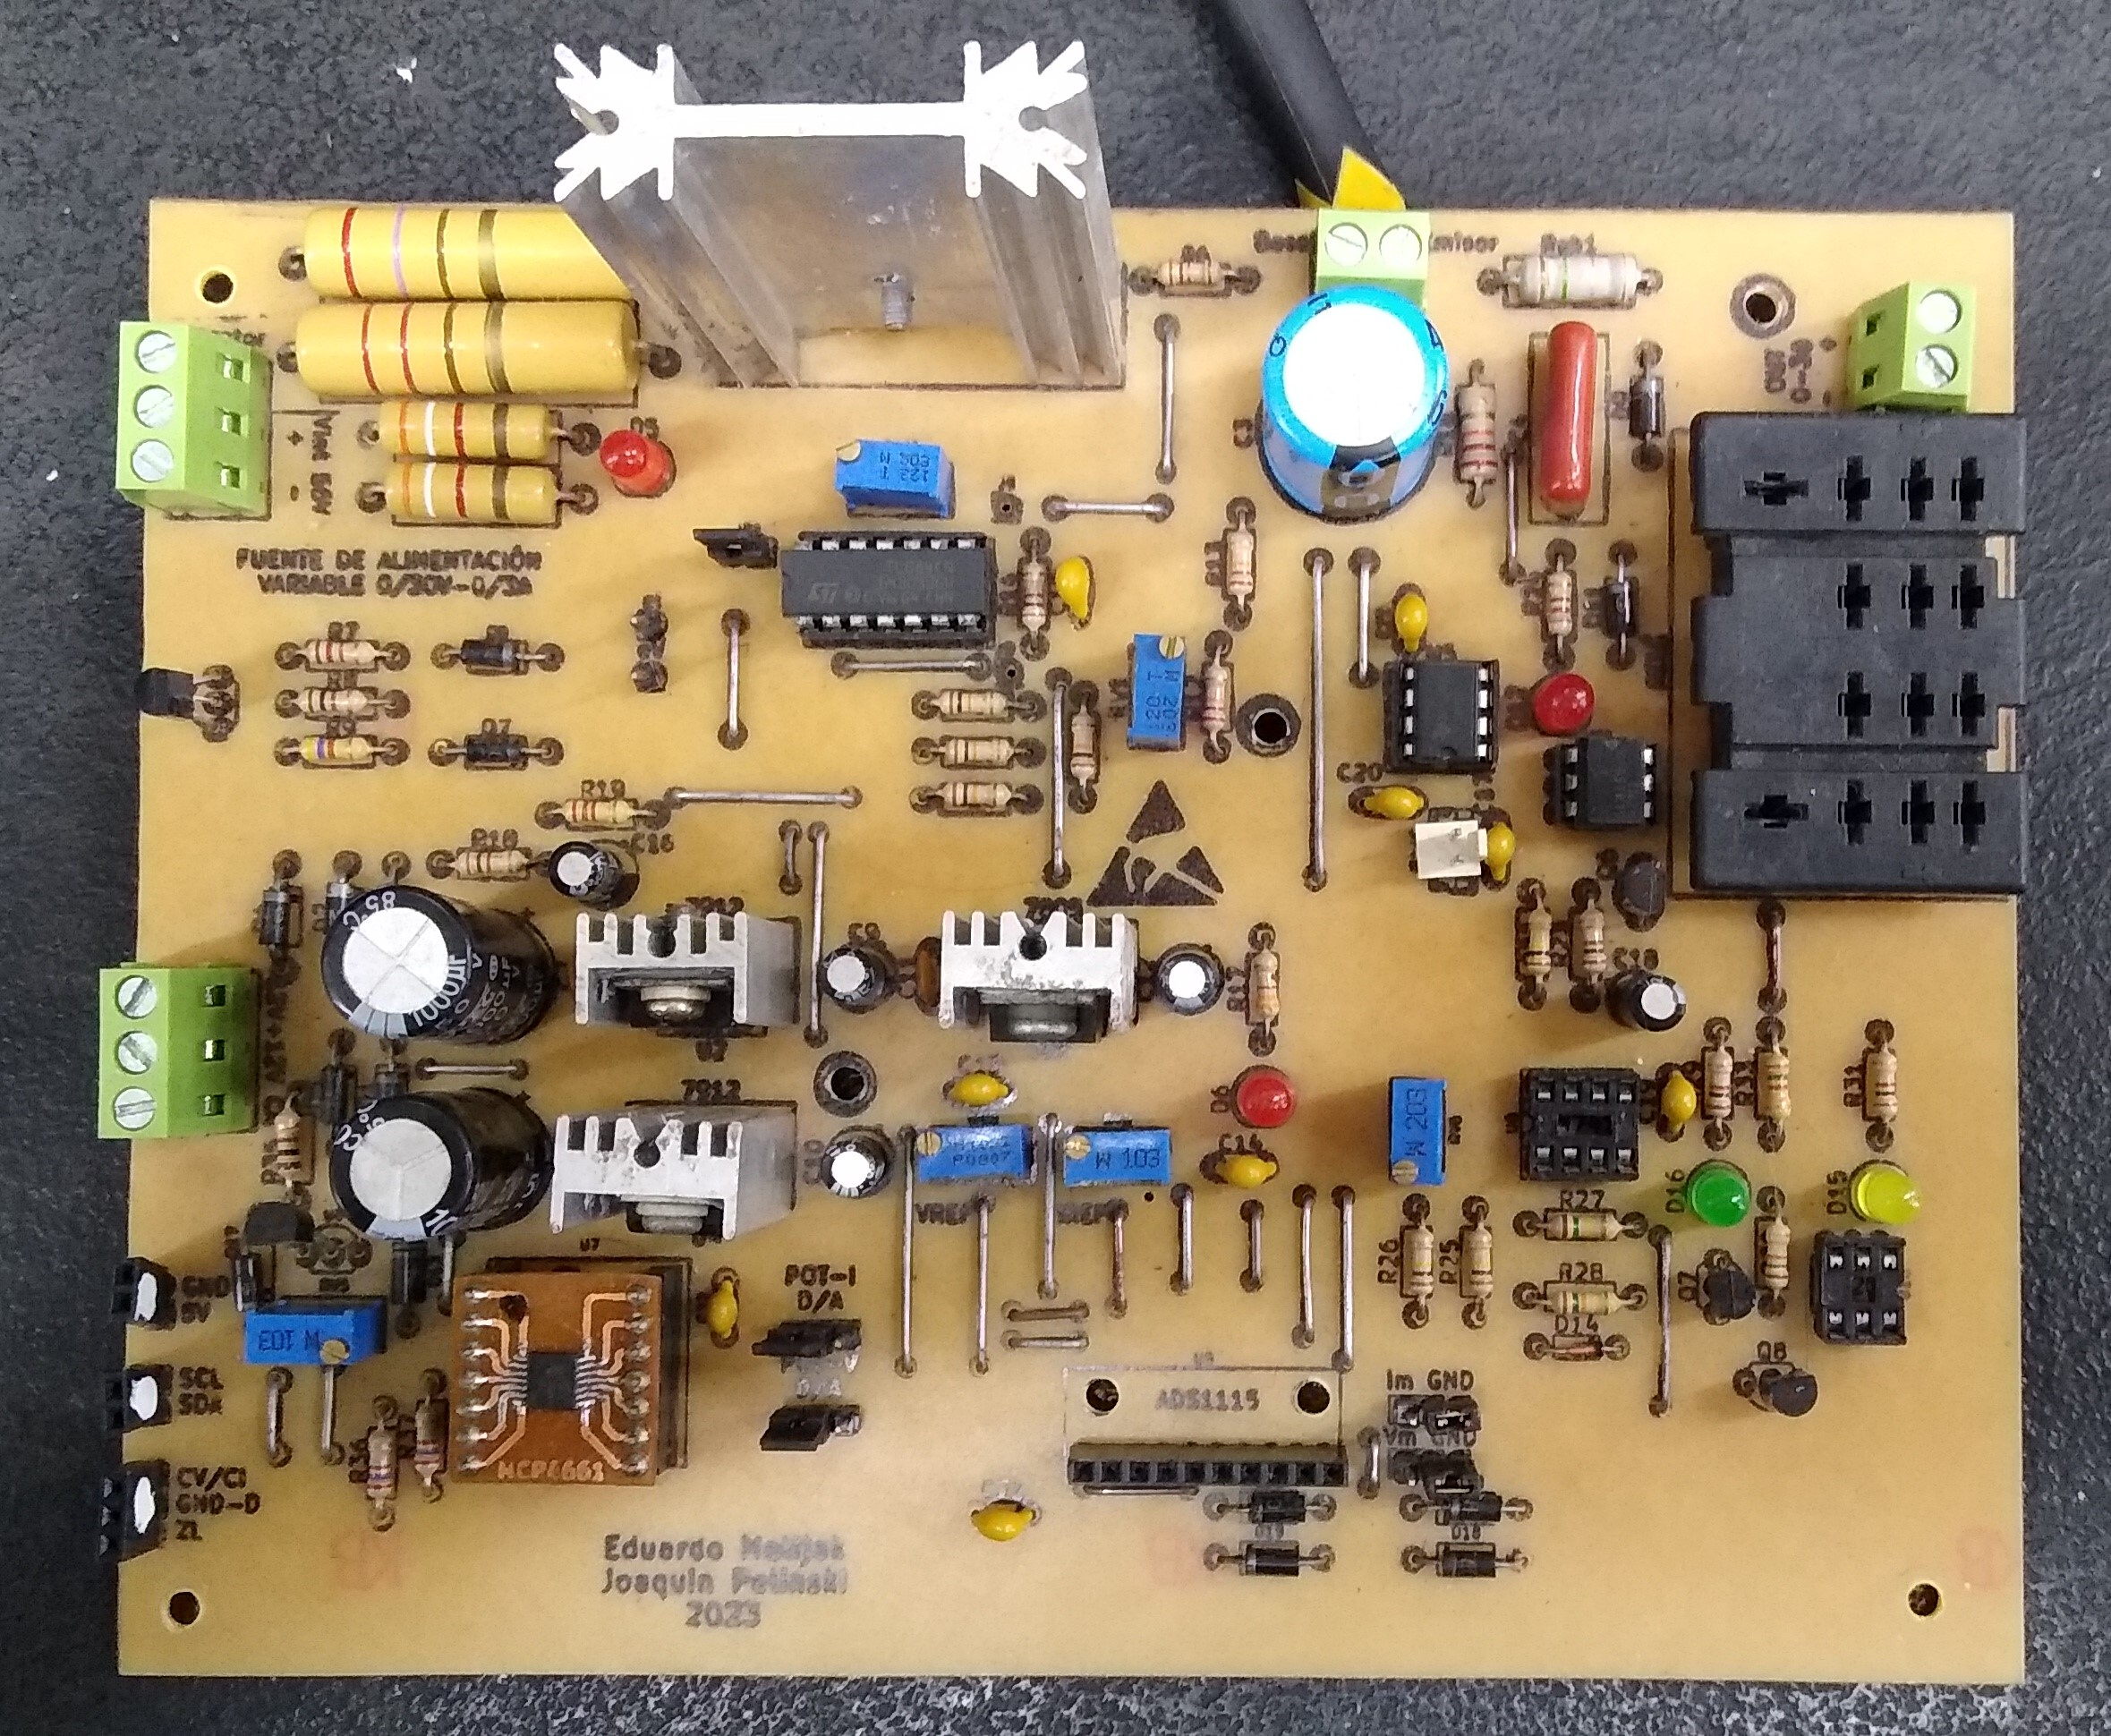
\includegraphics[width=0.8\textwidth]{./imagenes/fotos/placa_original.jpg}
    \caption{Antes del desmontaje de la placa de control analógica.}
    \label{F:placa_original}
\end{foto}

\begin{foto}[H]
    \centering
    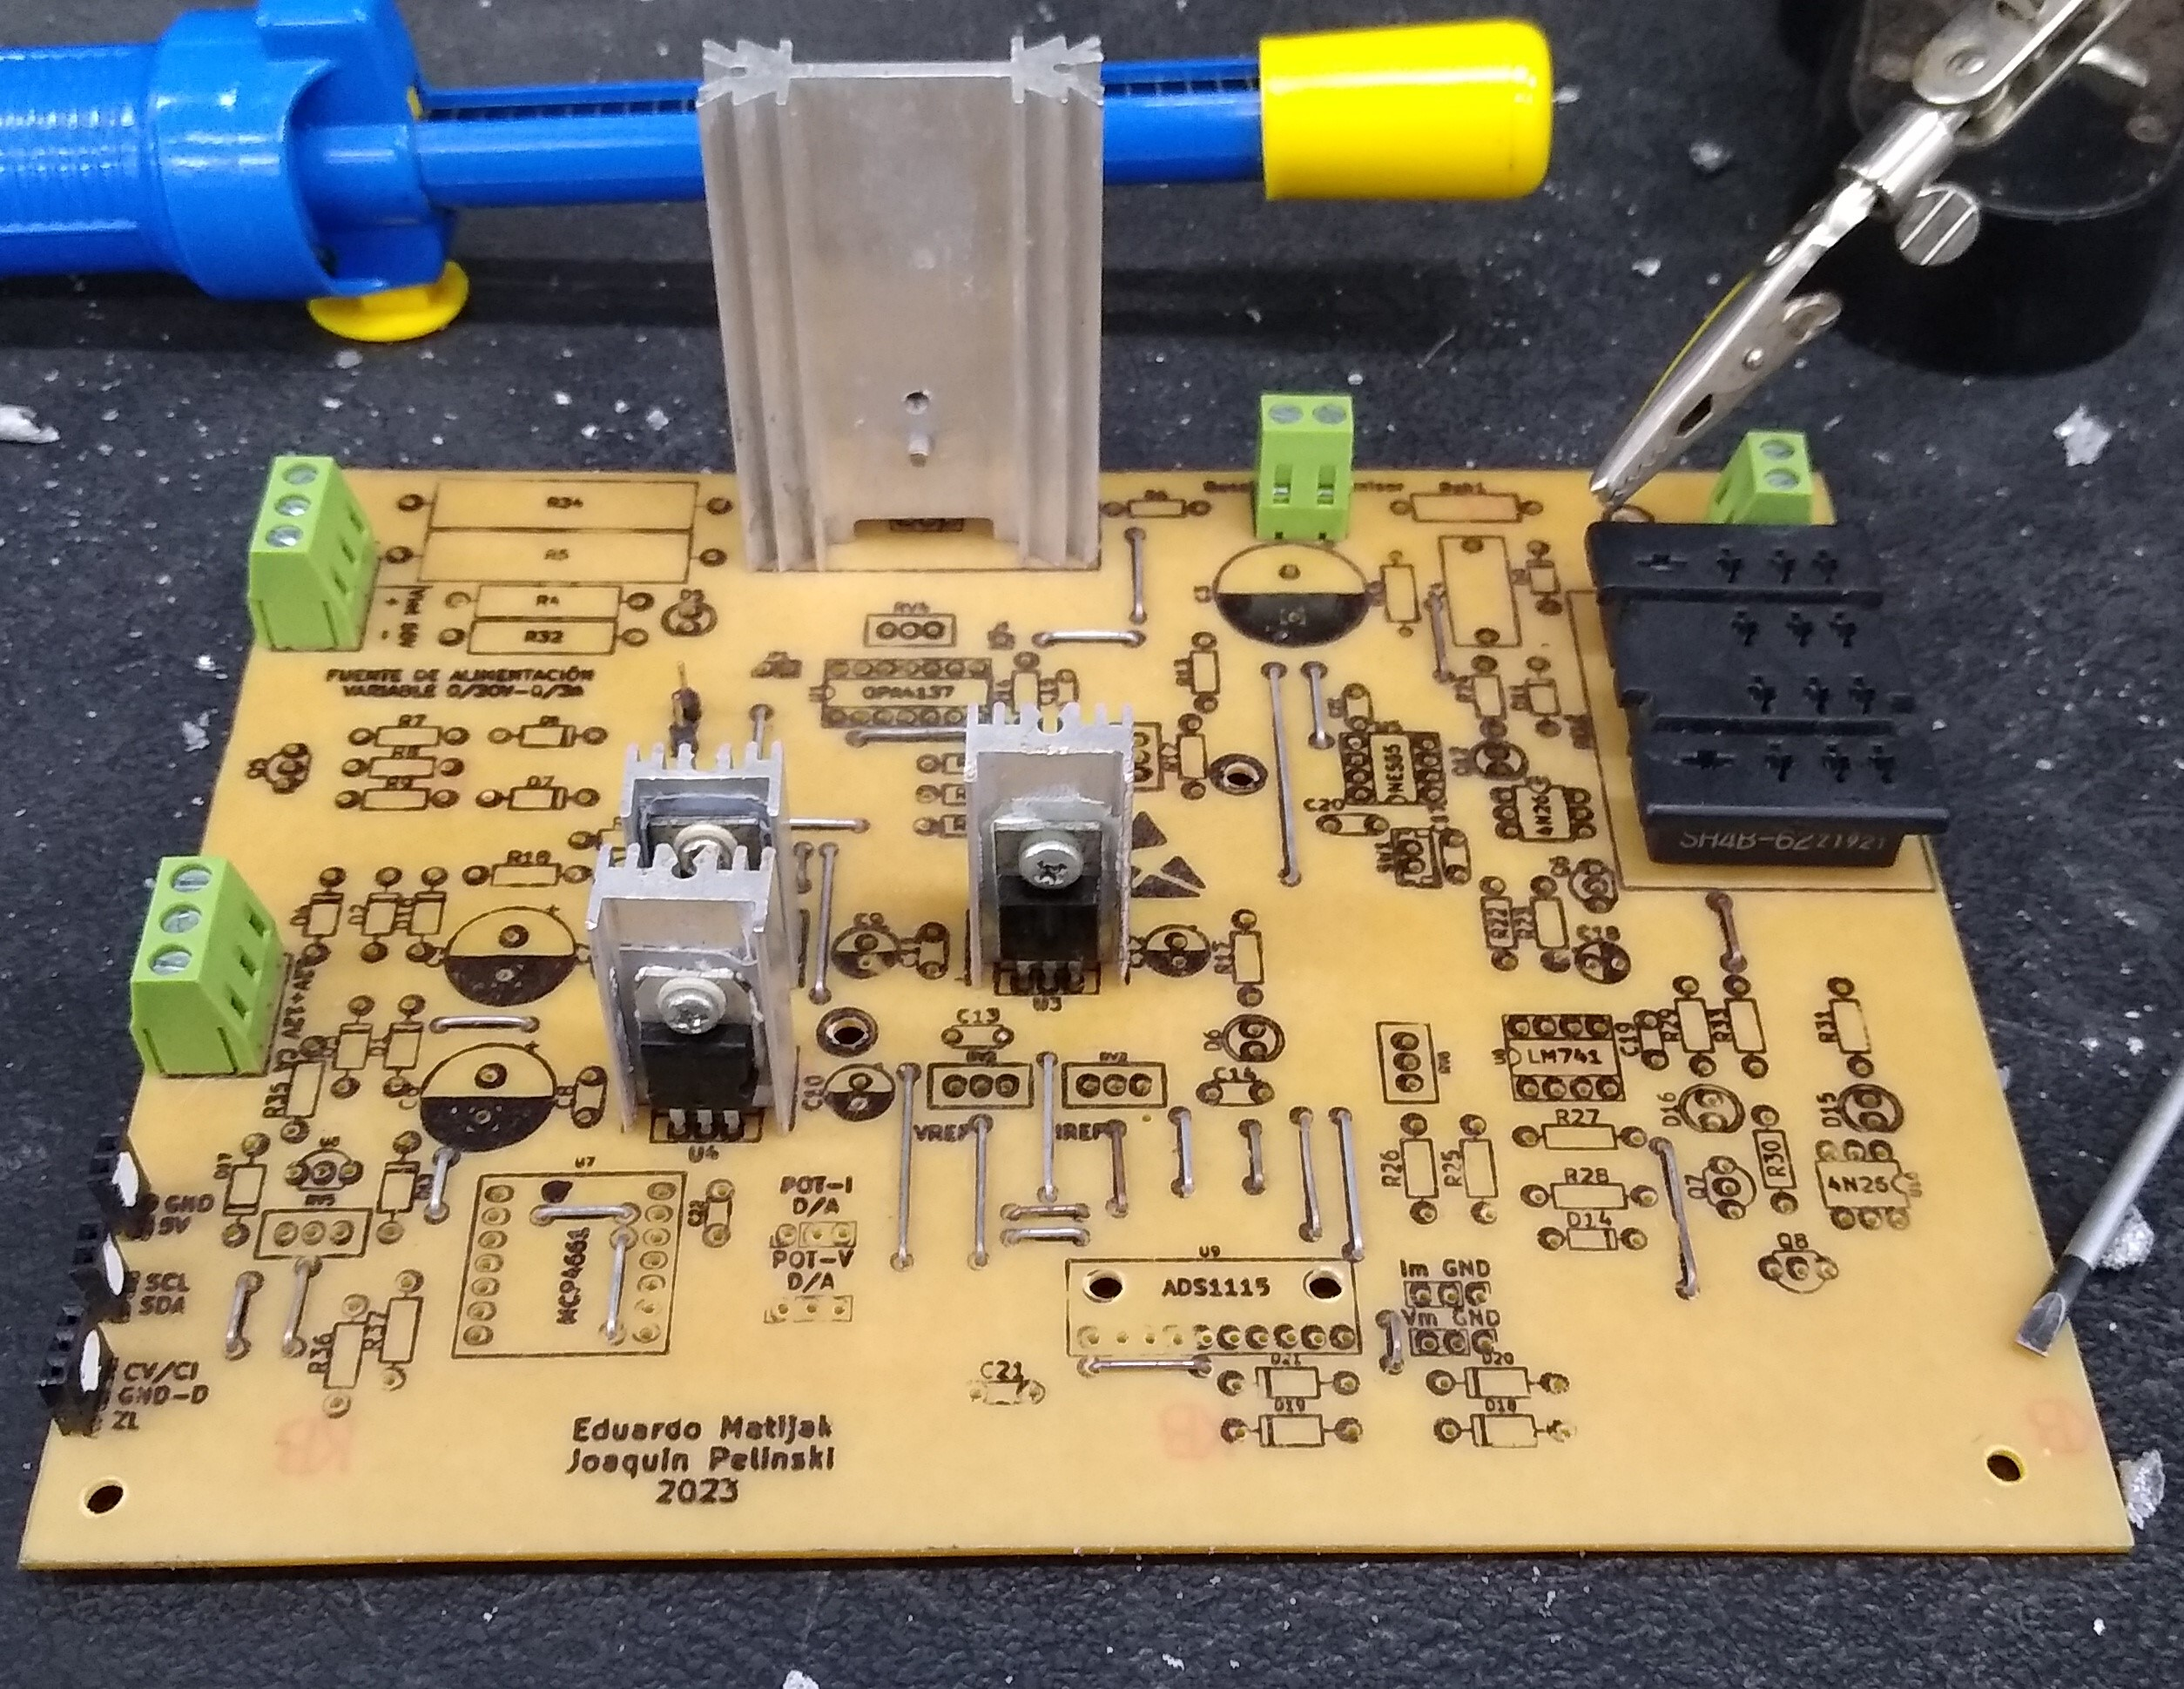
\includegraphics[width=0.8\textwidth]{./imagenes/fotos/desmontada.jpg}
    \caption{Después del desmontaje de la placa de control analógica.}
    \label{F:desmontaje_de_la_placa}
\end{foto}\par 

A continuación, se presenta el diseño del prototipo utilizado, el cual incorpora todos los elementos necesarios para la realización de las pruebas de funcionamiento. La característica principal de este PCB es su capacidad para integrar en un espacio compacto de 15x20 cm todos los componentes que anteriormente estaban dispersos en el modelo anterior. \par 
Una excepción notable en el diseño es la ubicación de la pantalla y el teclado, que se ha decidido mantener separados del PCB principal. Esta decisión se tomó debido a que no tendría sentido práctico incluir estos elementos directamente sobre la placa. En su lugar, se emplearon pines de salida, como borneras, para conectar estos componentes externos, facilitando su integración y operación. \par 
El diseño resultante, que se muestra en la Figura \ref{F:PCB_V1}, incluye también una representación tentativa en 3D del PCB. En esta representación se pueden observar las disposiciones de los componentes y la estructura general del prototipo. Es importante destacar que, para evitar daños y facilitar el acceso y reemplazo, algunos de los componentes están montados sobre tiras de pines hembra en lugar de estar soldados directamente sobre la placa. Esta configuración no solo mejora la durabilidad del prototipo, sino que también permite una mayor flexibilidad en la realización de pruebas y modificaciones. \par 

\begin{figure}[htbp]
    \centering
    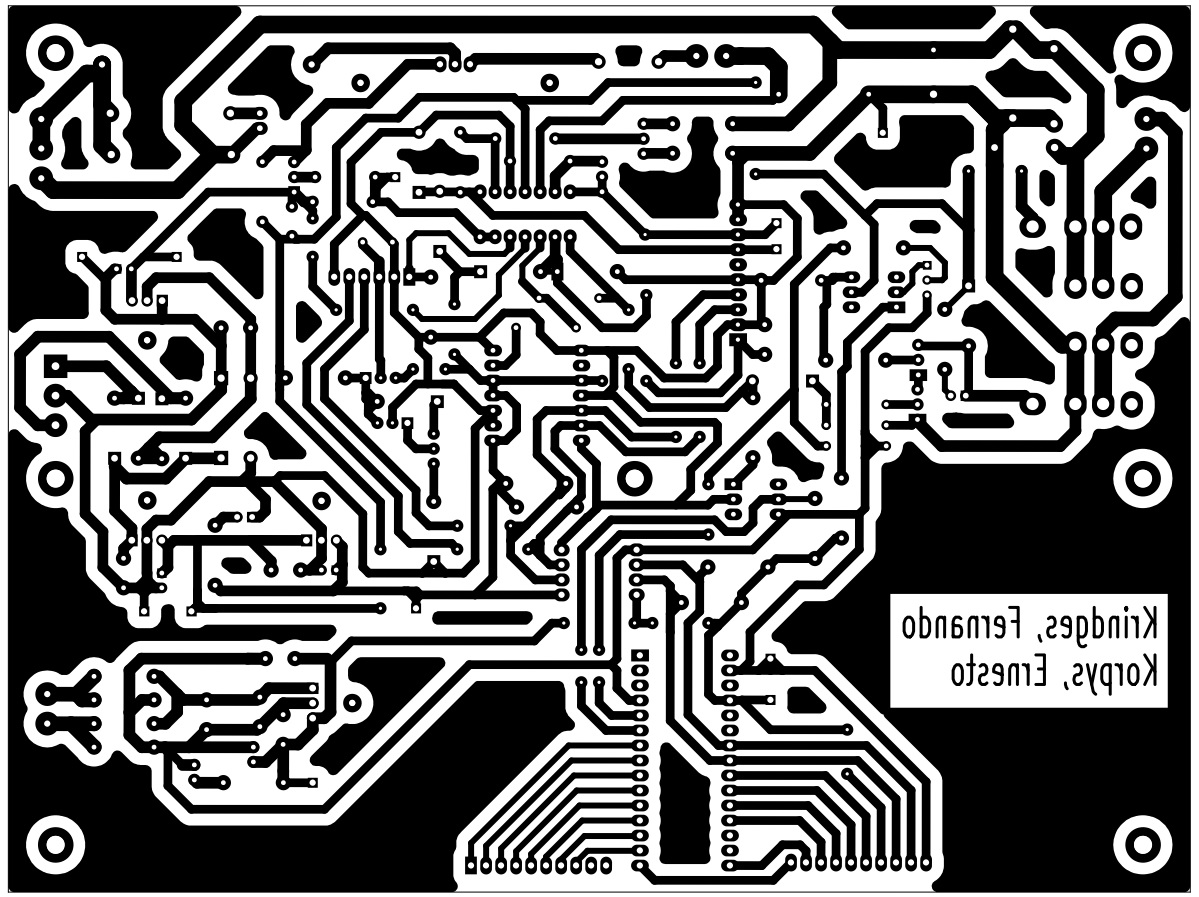
\includegraphics[width=\textwidth]{./imagenes/pcb_v1.jpg}
    \caption{Primer prototipo de PCB.}
    \label{F:PCB_V1}
\end{figure} \par

Se incluye un modelo 3D en el diseño con el fin de visualizar la disposición y la accesibilidad de los componentes, asegurando que el montaje y el mantenimiento del PCB sean lo más eficientes posible. Este es presentado en la Figura \ref{F:PCB_3D}.\par 
\begin{figure}[htbp]
    \centering
    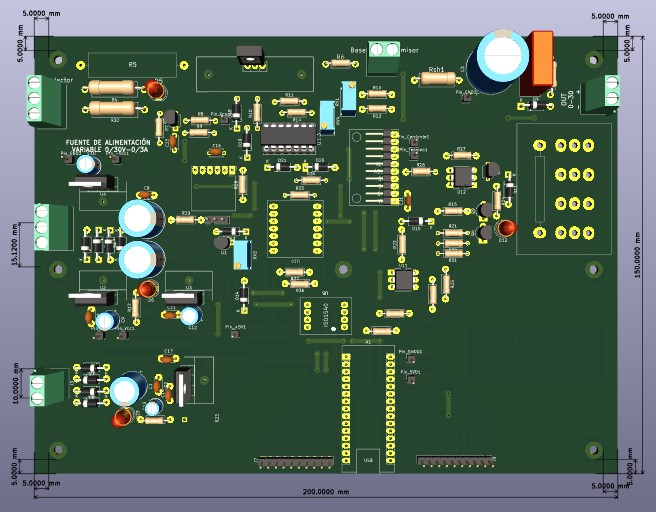
\includegraphics[width=\textwidth]{./imagenes/prototipo1.jpg}
    \caption{Vista 3D del primer prototipo.}
    \label{F:PCB_3D}
\end{figure} \par 

\begin{foto}[htbp]
    \centering
    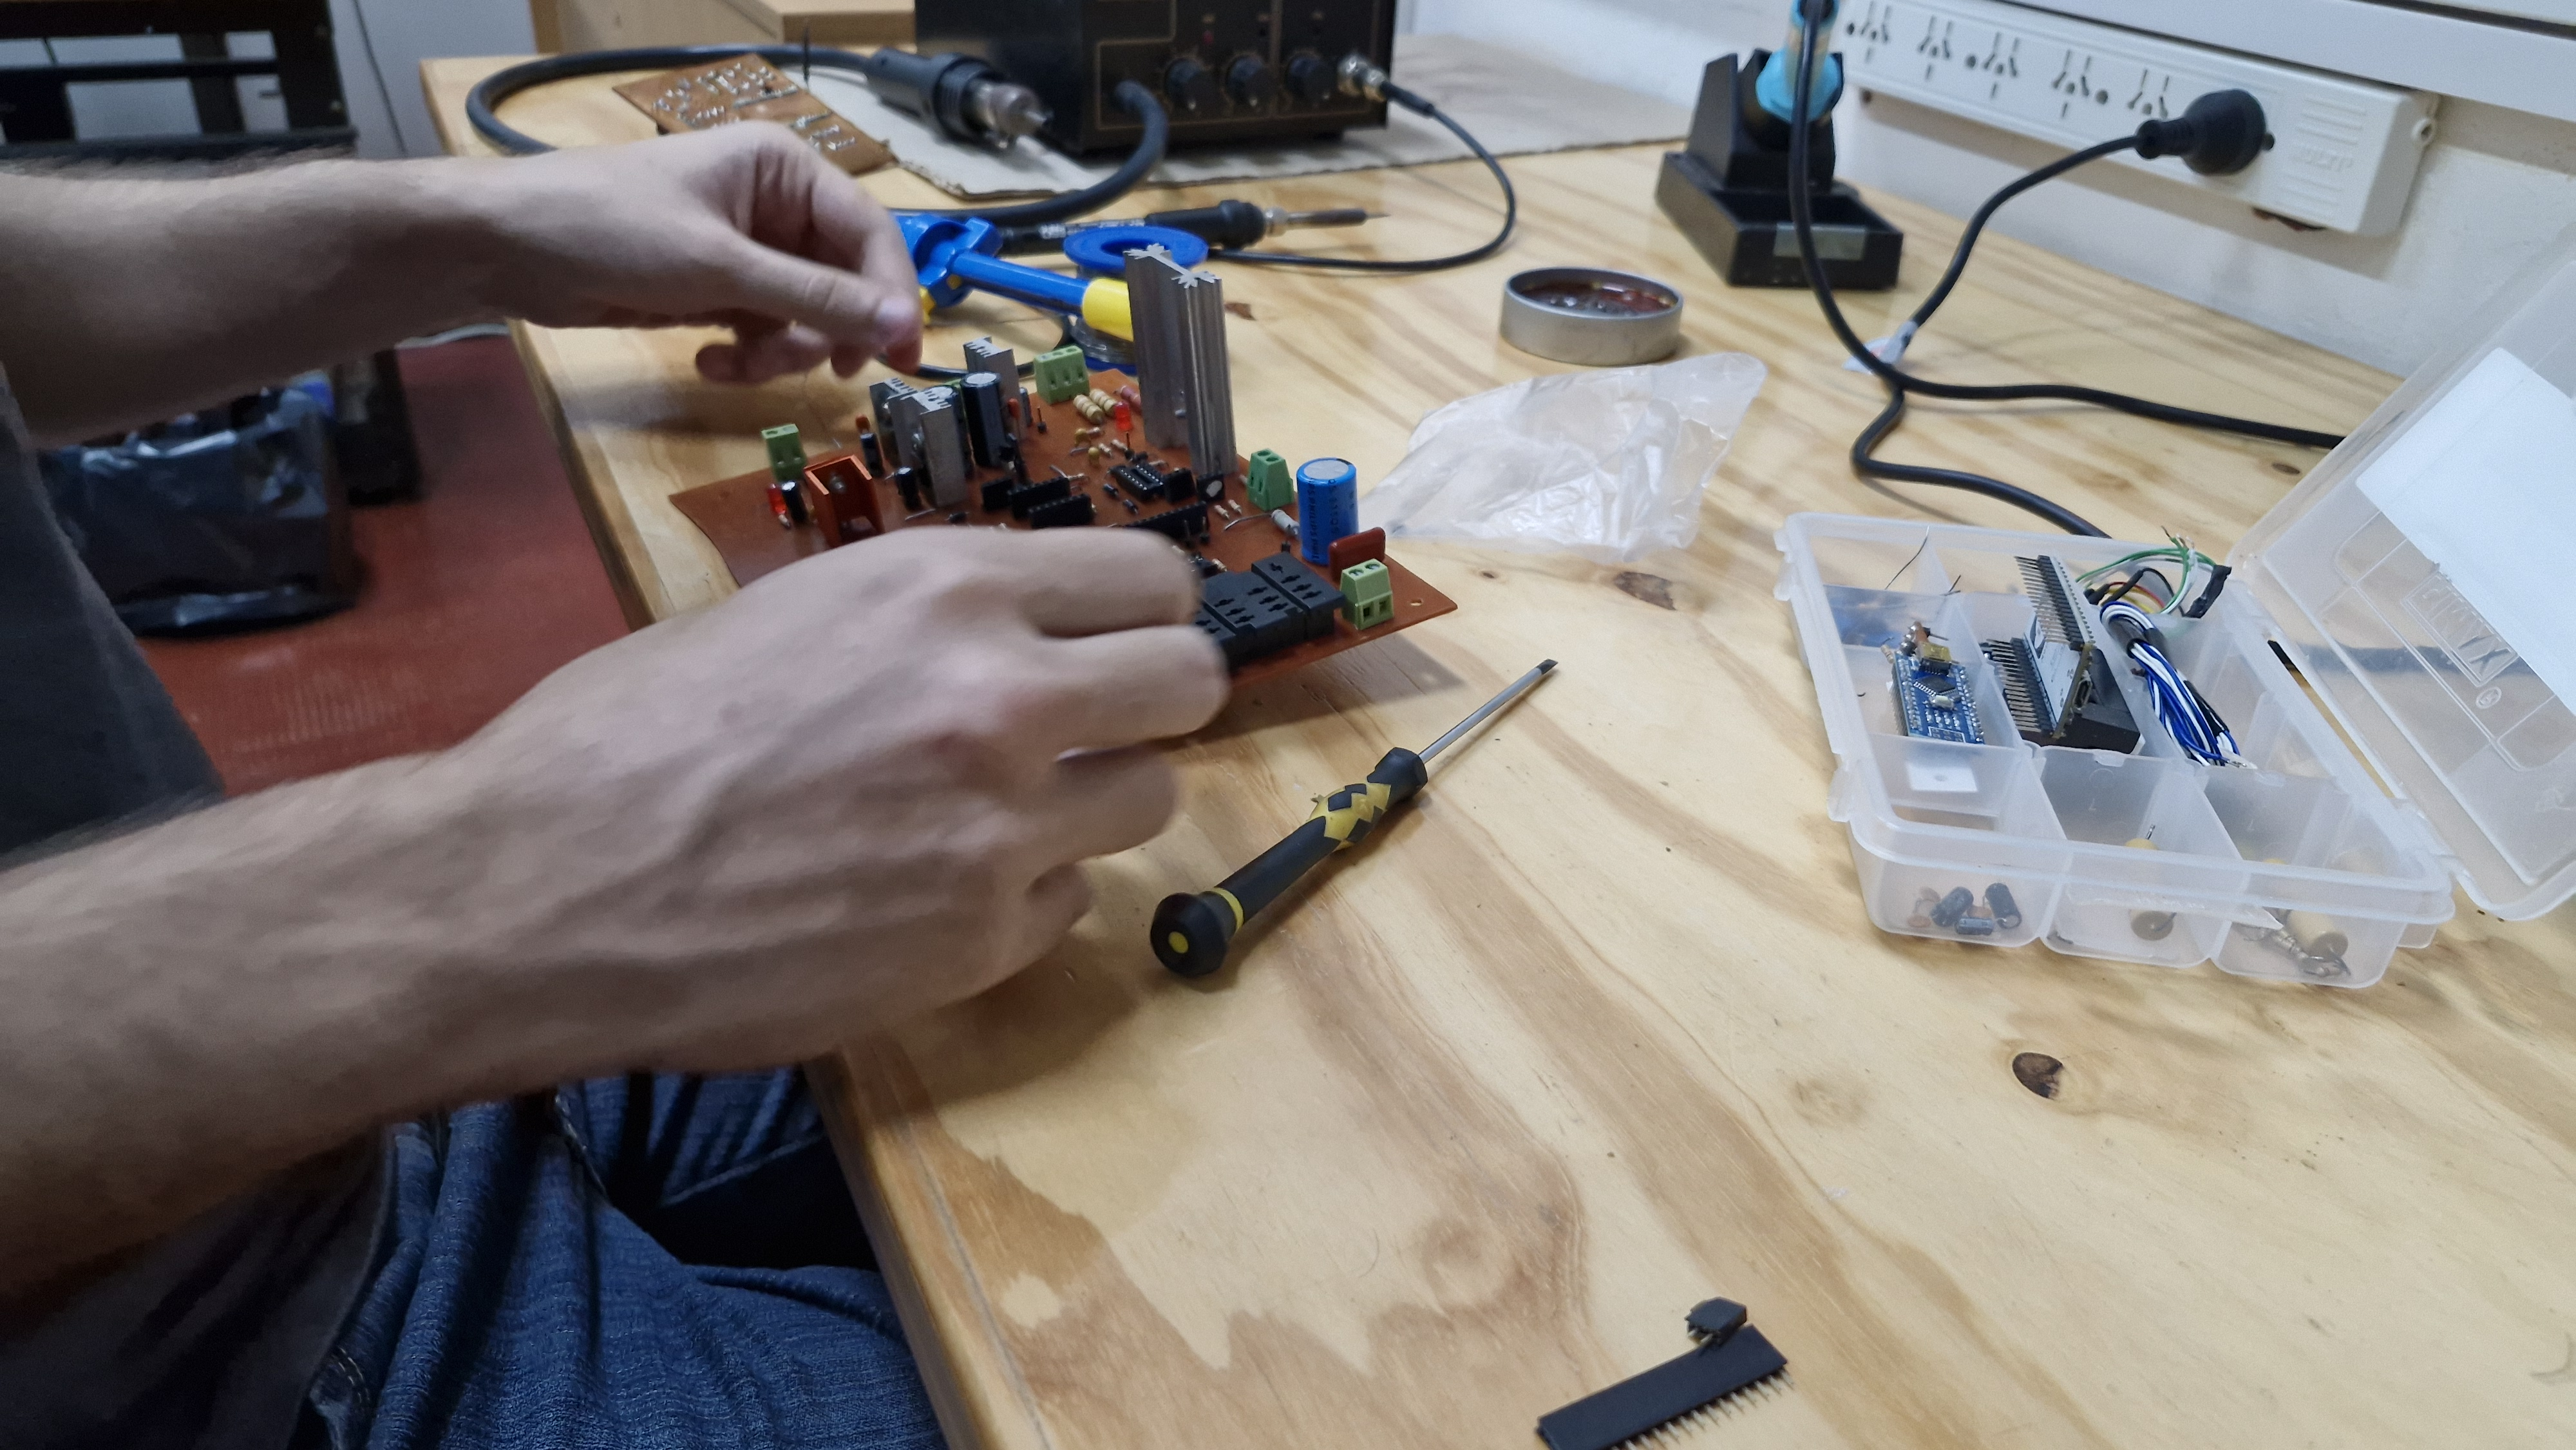
\includegraphics[width=\textwidth]{./imagenes/fotos/montaje.jpg}
    \caption{Montaje de los componentes en la placa.}
    \label{F:montaje_componentes}
\end{foto} \par 

\section{Primeras pruebas prácticas.}
Una vez verificada la continuidad de las pistas, el adecuado funcionamiento de los componentes, y los niveles de tensión en varios puntos clave, se procedió a energizar la fuente con todos los transformadores, tomando todas las precauciones necesarias para evitar daños a los componentes.\par 
A partir de este punto, se realizó una serie de pruebas y ajustes detallados para garantizar el correcto funcionamiento de la fuente. Estas pruebas incluyen la verificación de la respuesta del sistema bajo diversas condiciones de carga y la evaluación de la estabilidad del lazo de control. El uso del osciloscopio fue fundamental en este proceso, como se aprecia en la Fotografía \ref{F:esayos_y_pruebas}, ya que permitió observar en tiempo real cómo el lazo de control afectaba la salida de la fuente, aspecto crucial para el correcto desempeño del dispositivo.\par 
Durante estas pruebas, se monitorizaron diversos parámetros, tales como la tensión de salida, la respuesta transitoria, y el comportamiento ante variaciones en la carga. Cada ajuste se realizó con el objetivo de optimizar la \textit{performance} del prototipo, asegurando que este cumpliera con los requisitos especificados y operara de manera eficiente y estable.\par 

\begin{foto}[H]
    \centering
    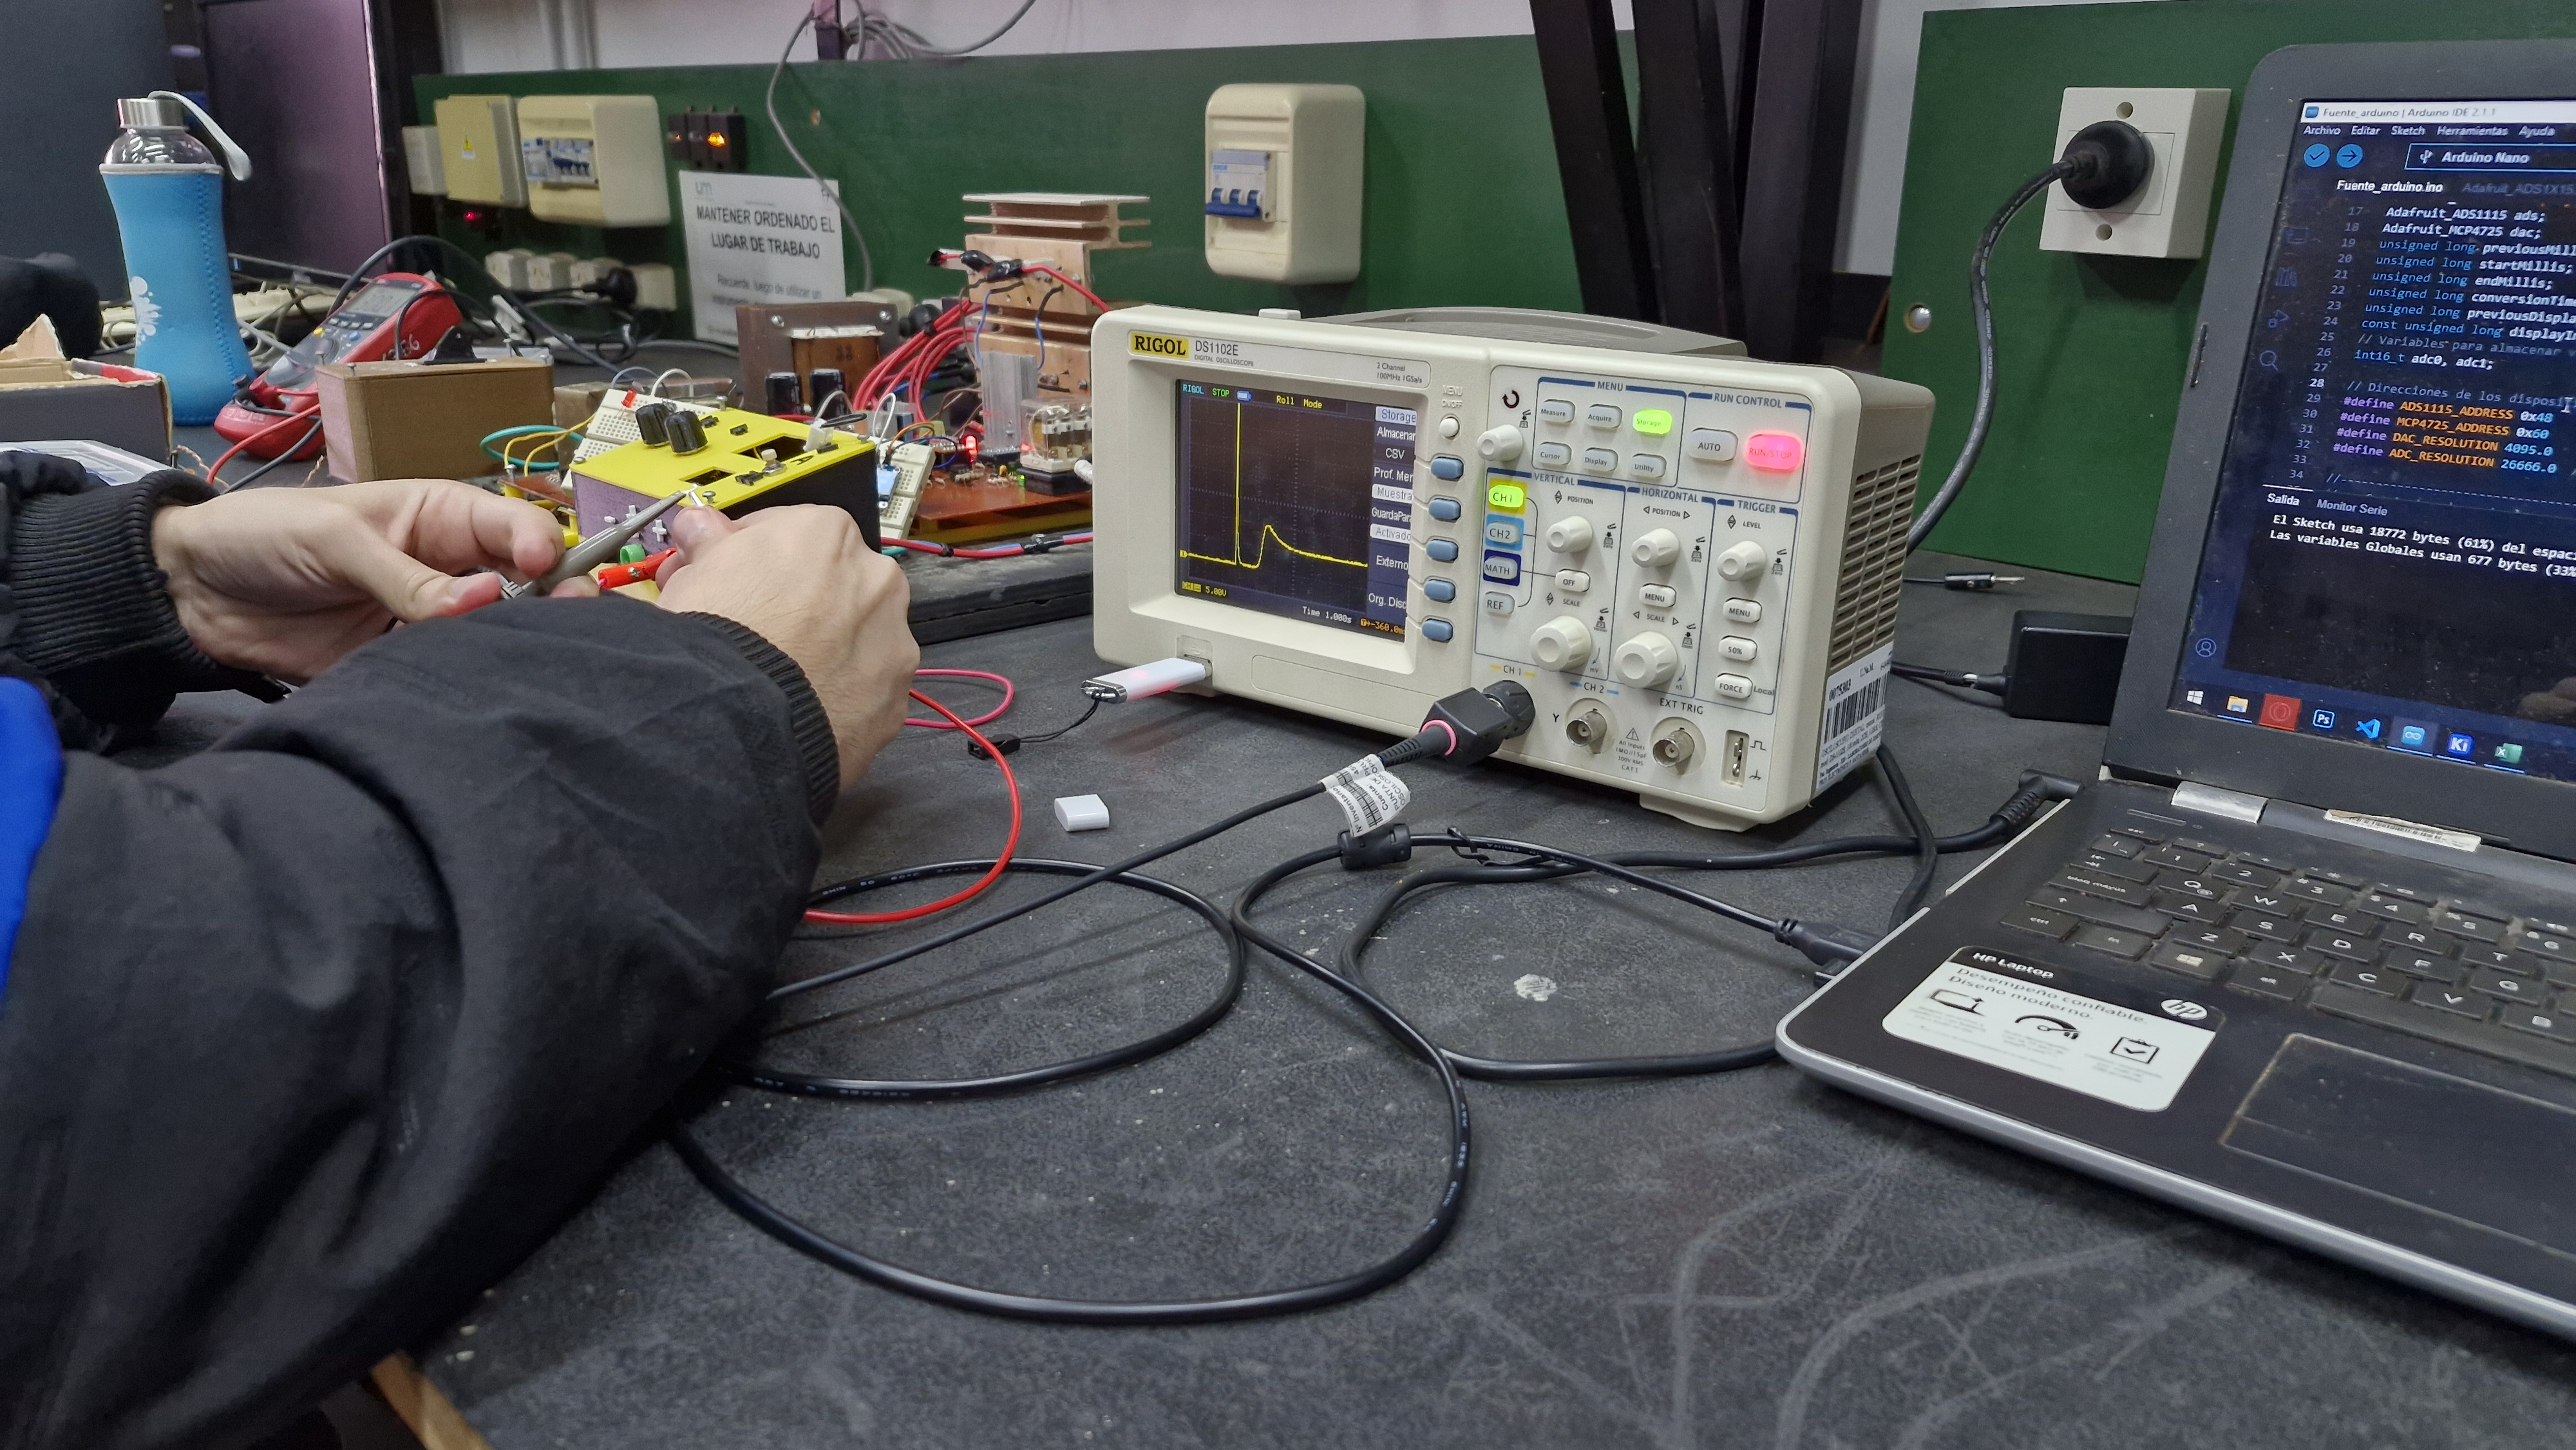
\includegraphics[width=0.9\textwidth]{./imagenes/fotos/osciloscopio.jpg}
    \caption{Ensayo con osciloscopio de la placa.}
    \label{F:esayos_y_pruebas}
\end{foto}\par 

\section{Resultados experimentales}
En esta sección, se presentan los resultados obtenidos del desempeño de la fuente de tensión bajo una condición de carga específica, prestando atención a su respuesta transitoria. Para ello, se utilizaron distintas configuraciones del controlador PID, cada una con distintas constantes $K_p$, $K_i$ y $K_d$, con el fin de estudiar cómo estas afectan el comportamiento dinámico del sistema.\par 

Las gráficas que se presentarán describen el comportamiento de la fuente de tensión durante el proceso de regulación, mostrando su respuesta ante la conexión de una carga. Durante estos ensayos registrados se utilizó un control ON-OFF para, de alguna manera, estabilizar la tensión de salida ante el estado de vacío. En cada uno de los gráficos se destacan los siguientes parámetros característicos de la respuesta transitoria:
\begin{itemize}
	\item \textbf{Tiempo de asentamiento ($t_s$)}: El tiempo necesario para que la respuesta permanezca dentro de un rango específico alrededor del valor final. Se utiliza para evaluar la rapidez de estabilización del sistema.
	\item \textbf{Sobrepaso($M_p$)}: La cantidad máxima que la señal de salida excede el valor de referencia. Este parámetro es clave para evaluar la estabilidad y robustez del controlador, ya que un sobrepaso elevado puede ser indeseable en sistemas críticos.
	\item \textbf{Error en estado estacionario}: Se analizará si, una vez estabilizada la señal, el valor final de la salida se aproxima adecuadamente al valor de referencia, o si existe un error residual que deba corregirse.
\end{itemize}\par 
Inicialmente, se presenta el gráfico que describe la respuesta del lazo de corriente en la figura \ref{F:Resultados obtenidos para el lazo de corriente}. Para el mismo se utilizan las siguientes constantes de control: $Ki_1=0,1$; $Ki_2=0,01$; y $Ki_3=0,001$. La resistencia de carga utilizada es de $100 \Omega$ y el valor de referencia utilizado es de $0,2A$. 
\begin{figure}[htbp]
    \centering
    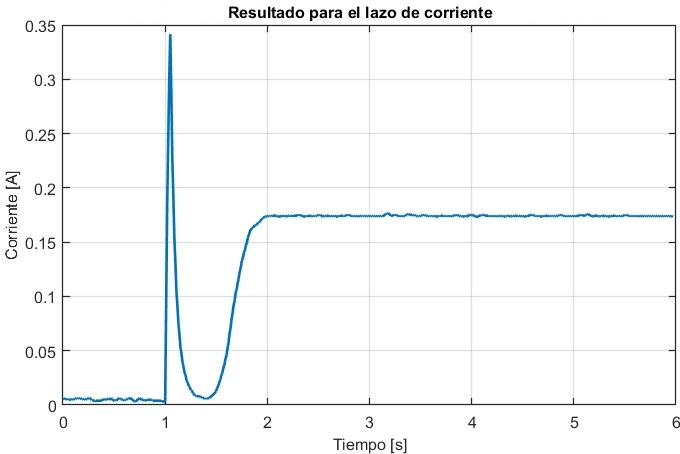
\includegraphics[width=0.9\textwidth]{./imagenes/NF5_lazo_corriente.jpg}
    \caption{Resultados obtenidos para el lazo de corriente.}
    \label{F:Resultados obtenidos para el lazo de corriente}
\end{figure}\par 
De la misma se observa una sobrecarga inicial, con un sobrepaso significativo en la corriente, llegando a aproximadamente $0,35A$. Este comportamiento se debe al control ON-OFF que se había implementado para controlar el voltaje en condición de vacío, dado que al momento de conectar la carga, el valor de tensión sobre la base del transistor resultó elevado. Tras el sobrepaso inicial, se observa una buena respuesta por parte del controlador, obteniendo una salida con un tiempo de asentamiento en torno a $0,5s$ y un sobrepaso casi nulo, verificando que las constantes para este lazo son adecuadas. El error en estado estacionario se debe principalmente a dos factores: se realizó una medición indirecta considerando que la resistencia de salida era de $100\Omega$ y faltó un ajuste fino en la calibración del ADC.\par 
A continuación, se presenta en la figura \ref{F:Resultados obtenidos para el lazo de tensión} los resultados obtenidos para el lazo de tensión. El valor fijado en este caso fue de $5V$ y nuevamente se empleó una resistencia de carga de $100\Omega$. Las constantes para el lazo de control utilizadas fueron: $Kv_1=0,0005$; $Kv_2=-0,0004$; y $Kv_3=0,0000001$.
\begin{figure}[htbp]
    \centering
    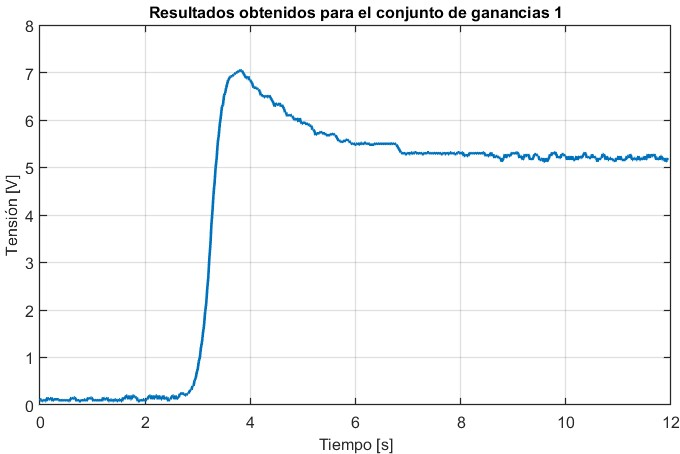
\includegraphics[width=0.9\textwidth]{./imagenes/NF3_tension_salida.jpg}
    \caption{Resultados obtenidos para el lazo de tensión.}
    \label{F:Resultados obtenidos para el lazo de tensión}
\end{figure}\par 
De la gráfica se observa una subida inicial, alcanzando un valor aproximado de $7V$para luego estabilizarse en torno a los $5V$ establecidos. El tiempo de asentamiento observado se encuentra alrededor de los $1,5s$. Es una buena aproximación para el primer conjunto de ganancias utilizado, sin embargo se requiere un poco de ajuste para disminuir el sobrepaso elevado que presenta.\par 

Finalmente, se presenta en la figura \ref{F:Resultados_3} los resultados obtenidos para un conjunto distinto de constantes de control para el lazo de tensión. Los valores utilizados fueron: $Kv_1=0,0005$; $Kv_2=-0,00032$; y $Kv_3=0,0000001$. En esta ocasión se fijó el valor de referencia a $15V$. 

\begin{figure}[htbp]
    \centering
    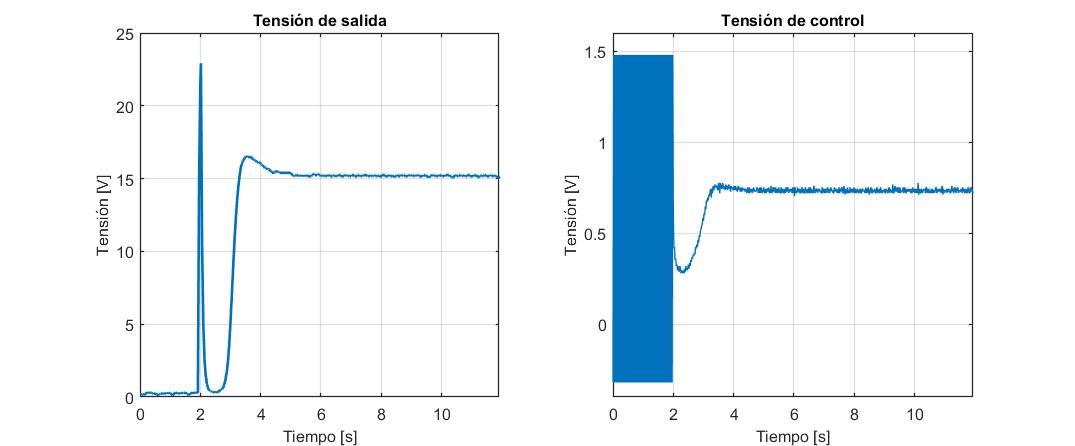
\includegraphics[width=0.9\textwidth]{./imagenes/NF10_tension_control.jpg}
    \caption{Respuesta de la tensión de salida y la tensión inyectada a la base de los transistores.}
    \label{F:Resultados_3}
\end{figure}\par 
Observando ambas gráficas se aprecia que el primer sobrepaso es sin dudas producido por el efecto del controlador ON-OFF al momento de conectar la carga. Luego, se produce un ligero sobrepaso de la tensión, siendo este aceptable para el valor configurado. El error en estado estacionario es muy cercano a cero, verificando una buena calibración de la medición de tensión además de un buen desempeño de la parte integral del control. \par 

El resultado de estos ensayos fue satisfactorio, evidenciando que el diseño y la construcción del PCB fueron exitosos pero sin embargo no del todo concluyentes. Por lo que para la construcción del siguiente prototipo, se obtuvieron las siguientes observaciones que serán tomadas en cuenta.  \par 


\section*{Observaciones}
\begin{itemize}
    \item Los transistores comienzan a operar con una acción de control mínima de $0,3V$.
    \item Ante condición de vacío el capacitor de salida se carga y dispara su voltaje en cuestión de unos milisegundos, por lo que es necesario un control especial para contemplar este detalle.
    \item Cuando el DAC se inicializa establece su voltaje de salida en $2,5V$. Luego de analizar su hoja de datos, es posible escribir en su memoria \entreComillas{EEPROM} el valor por defecto con el cual iniciará.
    \item Hubo un error en la asignación de la huella del DAC, teniendo dos de sus pines invertidos entre sí.
\end{itemize}

\section*{Mejoras a realizar}
\begin{itemize}
    \item Ajuste de constantes de controlador.
    \item Ajuste de frecuencia de muestreo.
    \item Mejora de la estrategia de control.
    \item Arreglar la huella y el \textit{ruteo} de las pistas relacionadas al DAC.
\end{itemize}

